\documentclass{standalone}
\begin{document}
	\setbeamerfont{block body}{size=\scriptsize}
	\setbeamerfont{block body example}{size=\scriptsize}
	\setbeamerfont{block body alerted}{size=\scriptsize}
	\begin{frame}{Training}{Centroid Estimation}
		\begin{block}{}
			\centering
			k-means clustering to find the centroids in the color space
		\end{block}
		
		\begin{columns}
			\begin{column}{.5\textwidth}
				
				\begin{block}{Clusters}
					\begin{itemize}
						
						\item Healthy Lung
						
						\item Edges
						 
						\item Bronchi
						
						\item Noise
						
						\item GGO and CS
						
					\end{itemize}
				\end{block}
			
			\centering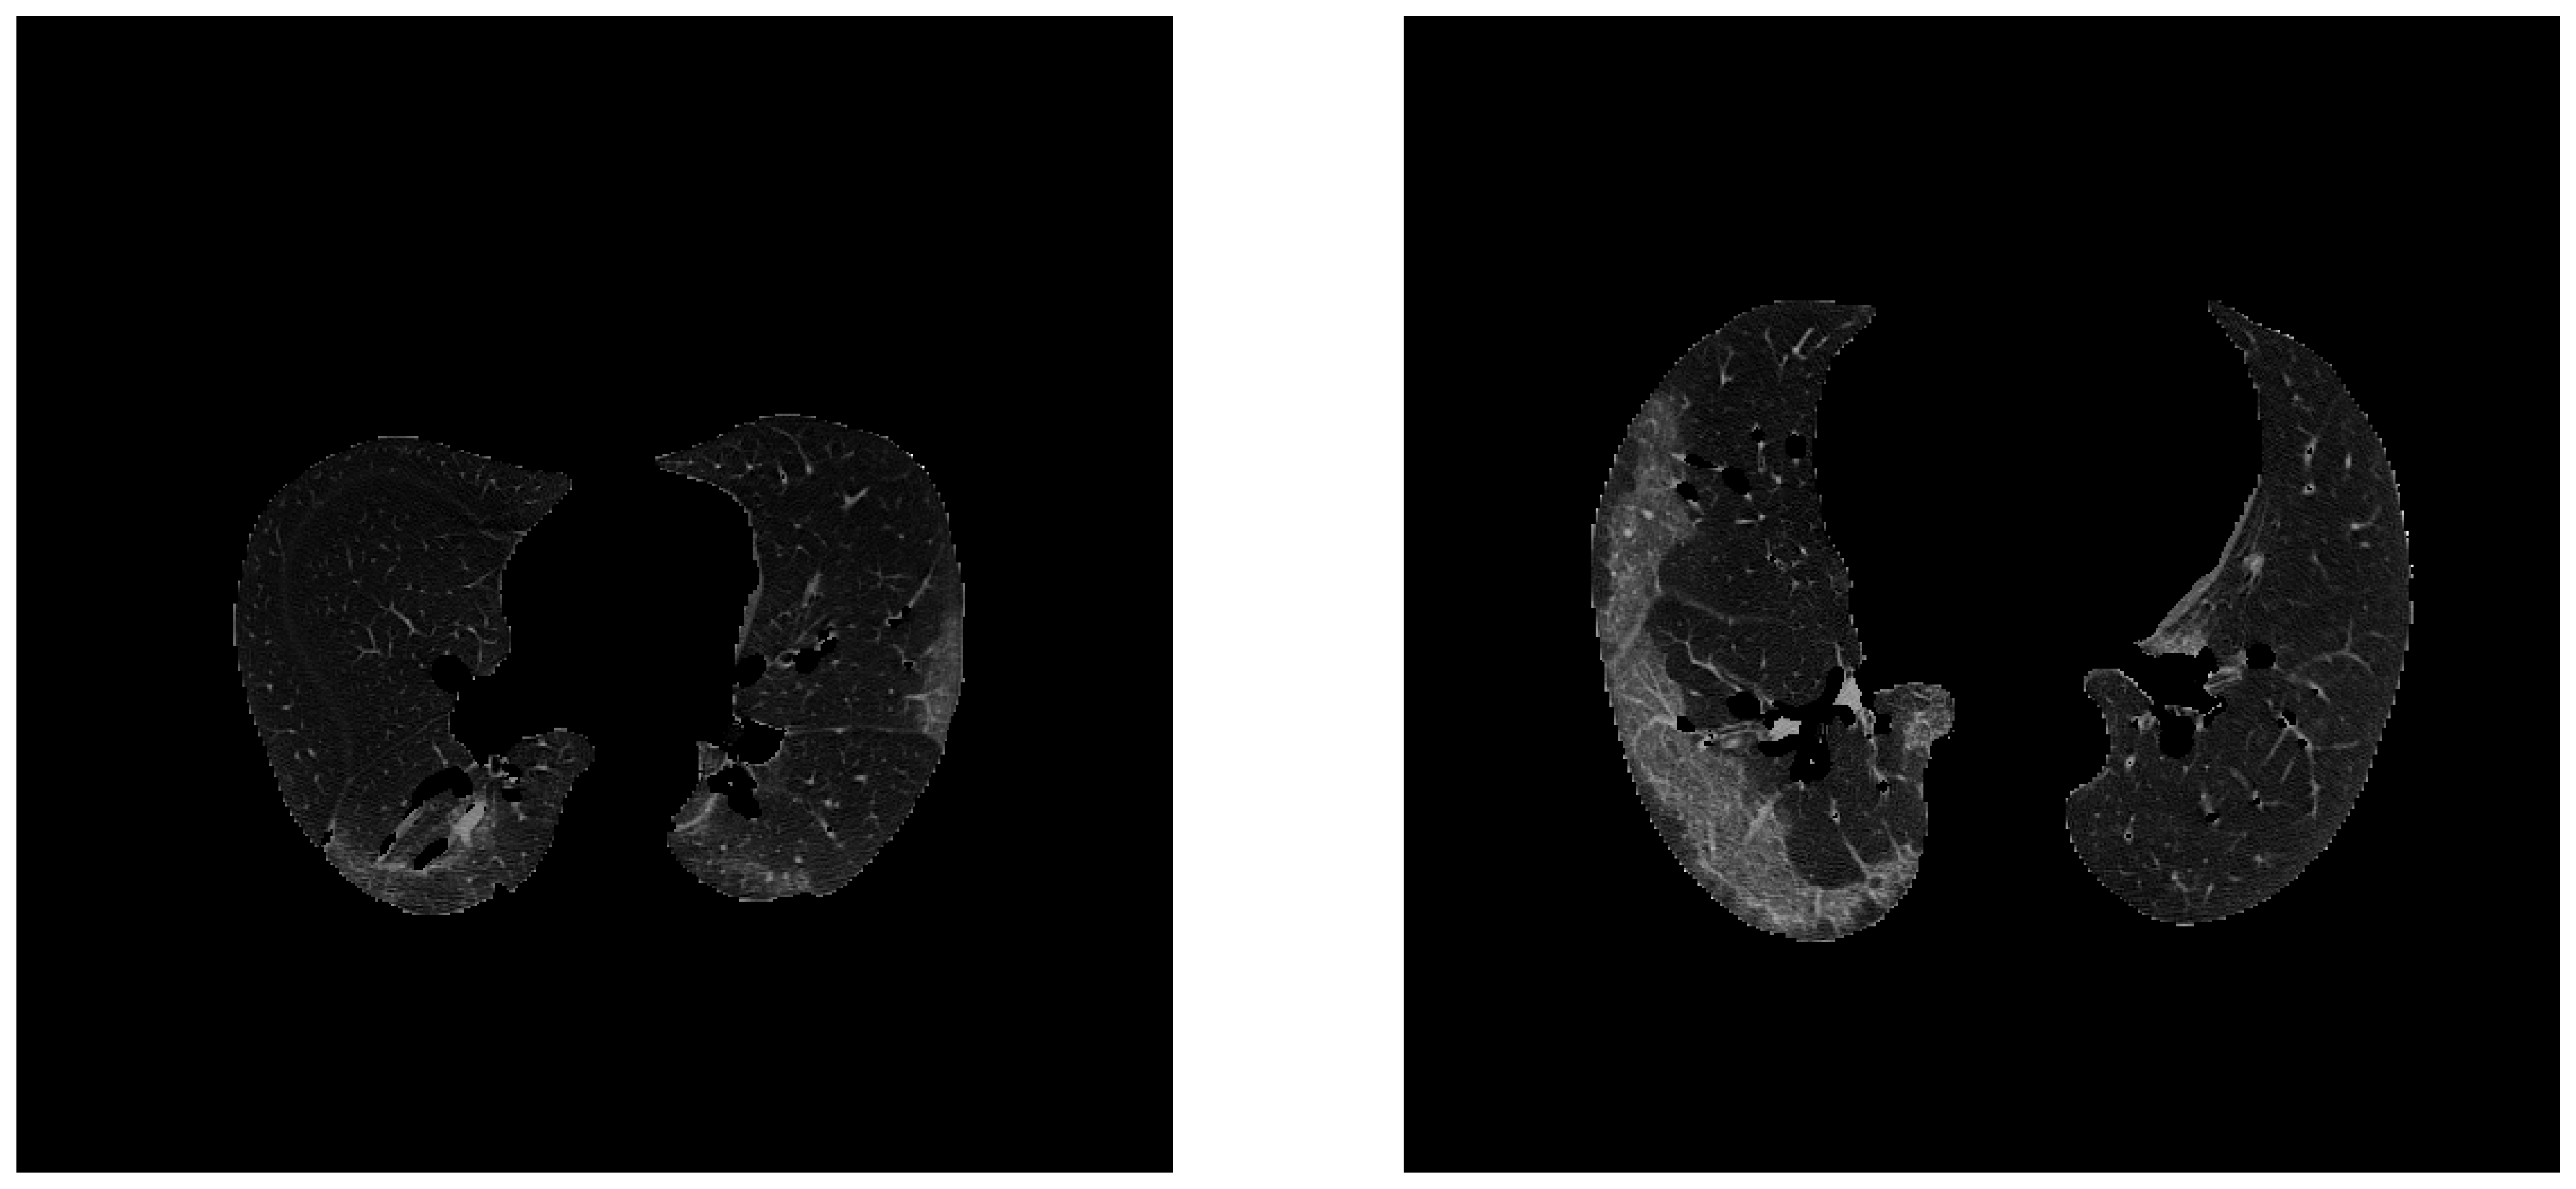
\includegraphics[width=\linewidth]{./img/ClusterRepr.png}
			\end{column}
		
			\begin{column}{.4\textwidth}
					\begin{alertblock}{Problem}	\setlength\itemsep{1.em}						
						\scriptsize{Non balanced cluster representation :} 
						\begin{itemize}
							\item Background :  Overrepresented
							
							\item GGO and CS: Can be under represented 
						\end{itemize}		
					\end{alertblock}
				
					\begin{exampleblock}{Solution}\setlength\itemsep{1.em}
						\begin{itemize}
							\item Remove Background
							
							\item Careful Selection of the Scans
						\end{itemize}
					\end{exampleblock}
			
			
			\end{column}
			
		\end{columns}
		
		
	\end{frame}
\end{document}